% chap4.tex (Definitions and Theorem)

\chapter{Simulations Study}
This section outlines simulation studies performed to analyze and investigate the source of overoptimism and how well the proposed methodology works in elevating this problem. To better understand the influences of adaptive methods on each stochastic components $\bar{y}_t$ and $s_t$, we generate training data $\mathcal{D}$ of size $n=500$ and test data set $\mathcal{D}'$ of size $n'=10,000$ from two nonlinear models in \citep{friedman1991multivariate} and one  true tree model;

%\subsubsection{Models}
%\begin{enumerate}[(A)]
%\item		
\begin{equation}
\label{eqn-modelA}
y \, = \,  -6 + 0.1 \exp(4x_1) + 4 \exp\{20(x_2 - 0.5)\} + 3 x_3 + 2 x_4 + x_5 + \varepsilon
\end{equation}
%	with $\varepsilon \sim \mathcal{N}(0, 1).$
%\item
\begin{equation}
\label{eqn-modelB}
y \, = \,  10\sin(\pi x_1 x_2) + 20(x_3 - 0.5)^2 + 10 x_4 + x_5 + \varepsilon
\end{equation}
%	with $\varepsilon \sim \mathcal{N}(0, 1).$
%\item	
\begin{equation}
\label{eqn-modelC}
y \, = \,  2 + 2\times sign(x_1 \leq 0.5) \times sign(x_2 \leq 0.5) + \varepsilon
\end{equation}
with $\varepsilon \sim \mathcal{N}(0, 1).$ and the $\mathbf{X_i}$'s are generated independently from random uniform[0,1] distribution of size $n = 500$.
%	\end{enumerate}	

Model (\ref{eqn-modelA}) has a nonlinear additive structure on the first two variables and a linear term on the last three variables \citep{friedman1991multivariate}. Model (\ref{eqn-modelB}) has a nonlinear additive with the first two variables having a multiplicative parabolic interaction term, the third variable with a quadratic relation, and the final two variables with a linear dependence \citep{friedman1991multivariate} and the true tree model is given by model (\ref{eqn-modelC}). For simplicity, model equations 4.1, 4.2, and 4.3 would be denoted as models A, B, and C respectively.
%	\end{enumerate}              
       
With each given model, a best-sized tree $\mathcal{T}$ is then constructed via pruning and cross-validation with the 1-SE rule \citep{breiman1984classification}. For each terminal node, $\bar{y}_t$ and $s_t$ are extracted. Then we generate another independent test data set $\mathcal{D}'$ of size $n'=10,000.$ Send $\mathcal{D}'$ down to tree $\mathcal{T}$ and recompute the node mean and SD $(\bar{y}'_t, s'_t).$ Mean values of $\bar{y}_t$, $s_t$, $\bar{y}'_t$ and $s'_t$ are computed as indicated in Table \ref{table:1}

\vspace{0.1in}
\begin{table}[H]
\caption{ Mean values, Influence of tree modeling on inference on node averages $\bar{y}_t$ and node SD $s_t$ for $t \in \widetilde{T}$ computed with training data $\mathcal{D}$ and test data $\mathcal{D}'$. }
	\centering
\begin{tabular}{ |p{1cm}|p{3cm}|p{3cm}|p{3cm}| p{3cm}|}%p{2cm}|p{2cm}|p{2cm}|p{2cm}|}
	\hline
	Tree   &$\bar{y}_{t}$ &$s_t$& $\bar{y}_{t}'$ & $s_t'$\\
	\hline
	1&	7.05608&	1.328307&	7.089057&	1.50636\\

	2&	6.813485&	1.335768&	6.785658&	1.471886\\

	3&	6.559332&	1.226844&	6.597213&	1.43782\\

	4&	6.72372&	1.220396&	6.691766&	1.437119\\

	5&	6.990564&	1.362192&	6.88289&	1.480317\\
	
	\vdots & \vdots & \vdots & \vdots & \vdots\\
	
	96&	6.818623&	1.232034&	6.895311&	1.457672
\\
	97&	6.435047&	1.206669&	6.425234&	1.467036
\\
	98&	7.006038&	1.285327&	6.986894&	1.503891
\\
	99&	6.904065&	1.218327&	6.846934&	1.422443
\\
	100	&6.878547&	1.219453&	6.752506&	1.379429\\
	\hline
\end{tabular}
\label{table:1}
\end{table}
It is observed from Table \ref{table:1} given by equation model \ref{eqn-modelA} that, on average $\bar{y}_t$ and~$\bar{y}'_t$ has a correspondence to each other that is to say they match well in figures. However, the SDs exhibits some variations in figures, i.e, $s_t'$ from the test data is much greater than that of the training data as indicated in Table \ref{table:1}. These average $s_t$ values clearly support the vast variation in the standard deviations resulting in the downwards biasedness as depicted in figure \ref{fig-inf-influence}. This observation further strengthened our motivation for the study.

%\section{Existing Method }
\section{ Bootstrap Calibration (BC)}
With the existing methodology BC and its outlined algorithm. We simulated data from the three models and use Algorithm \ref{Alg-BC} to obtain the coverage probabilities. Even though the population $\alpha$ is rarely known in practice, by simulation we exploit the luxury of data availability in the simulation setting and obtain an estimate of $\alpha$ by generating large test samples evaluation of the bootstrap calibration approach to aid our evaluation of the bootstrap calibration approach.% comparison with the bootstrap calibrated alpha.

For each model configuration, we started by generating a training data $\mathcal{D}$ of size $n=500$ and also test data set $\mathcal{D}'$ of size $n'=500$. A set of $\alpha \in [{1: 0.005}]$ are chosen. With the training data $\mathcal{D}$, a best-sized tree $\T$ is then constructed via pruning and cross-validation with the 1-SE rule \citep{breiman1984classification} and the estimates $\{(n_t, \bar{y}_t, s_t): t \in \widetilde{\mathcal{T}}\}$ \ for all terminal nodes of $\T$ are recorded. Send $\mathcal{D}'$ down to $\T$ and recomputing $\{ \bar{y}_t': t \in \widetilde{\mathcal{T}}\}$ \ for all terminal nodes of $\T.$ Now are we construct $(1-\alpha_k) \times 100\%$ CI in node $t$ for $\bar{y}_t$ based on set coverages $\alpha$. If $\bar{y}_t'$ $\in$ $(L_{tk}, U_{tk}) \in (\bar{y}_t' \pm z_{1-\alpha/2} \, \frac{\displaystyle s_t}{\displaystyle \sqrt{n_t}}$), then we record the $\alpha's$ for which $\bar{y}_t'$ $\in$ $(L_{tk}, U_{tk}) \in (\bar{y}_t' \pm z_{1-\alpha/2} \, \frac{\displaystyle s_t}{\displaystyle \sqrt{n_t}}$)  for every mean node as the population coverage probabilities.\newline
Similarly, we take $B$ bootstrap samples $\{ \mathcal{D}_b: b=1, \ldots, B\}$, such that for each bootstrap sample $\mathcal{D}_b$, a best-sized tree $\T_b$ is constructed  via prunning and cross validation to obtain the estimates of $\mathcal{T}_b$ as $\{(n_t, \bar{y}_t, s_t): t \in \widetilde{\mathcal{T}}_b\}$ \ for all terminal nodes of $\T_b.$

Sending $\mathcal{D}$ down to $\T_b$ and recomputing $\{ \bar{y}_t': t \in \widetilde{\mathcal{T}}_b\}$ \ for all terminal nodes of $\T_b$, a $(1-\alpha_k) \times 100\%$ CI in node $t$ for $\bar{y}_t'$ based on set coverages $\alpha$ is then constructed. If $\bar{y}_t'$ $\in$ $(L_{tk}, U_{tk}) \in (\bar{y}_t' \pm z_{1-\alpha/2} \, \frac{\displaystyle s_t}{\displaystyle \sqrt{n_t}}$), then we record the $\alpha's$ for which $\bar{y}_t'$ $\in$ $(L_{tk}, U_{tk}) \in (\bar{y}_t' \pm z_{1-\alpha/2} \, \frac{\displaystyle s_t}{\displaystyle \sqrt{n_t}}$) for every mean node as the bootstrap coverage probabilities. A plot of comparison for the population and bootstrap coverage probailities obtained in Figure \ref{fig-Trial-IBC}.


\begin{figure}[H]
	\centering
	\includegraphics[scale=0.50, angle=270]{fig-Trial-I.eps}
	\caption{Coverage plot of the calibrated alpha against population alpha.} 
		\label{fig-Trial-IBC}
\end{figure}
\vspace{0.1in}
From Figure \ref{fig-Trial-IBC}, the dash line serves as a reference line with $(1-\alpha)= 0.95$. Given the plot, our goal is that the calibrated (bootstrapped) alpha ($\alpha'$) should mimic that of the unknown population alpha ($\alpha$) and their intersection points with the reference line should be close to each other. The graphical output indicates that model A and model B do not show our desire result, thus the bootstrap calibrated alpha is too liberal compared to the population alpha which is not good. The third model which is the true tree model shows good results, this is because its a true classification model. Hence the existing methodology BC becomes too radical to tackle the issue of making a valid inference with decision trees. A more conservative approach than BC is needed.



\section{Proposed Method }
\subsection{ Bias Correction on SD}
Here we experimented again with the bootstrap correction approach in algorithm(\ref{Alg-bias-sd}) using the three model configurations. With each given model, we generated training data $\mathcal{D}$ of size $n=500$ and test data set $\mathcal{D}'$ of size $n'=10,000$ with bootstrap sample $\mathcal{B}$=500. %and found that it works exceptionally well as illustrated below. 

\subsubsection{ Model A}
\vspace{0.1in}
\begin{table}[H]
	\caption{Table of result for biased corrected SD computed with training data $\mathcal{D}$ and test data $\mathcal{D}'$.  }
	\begin{tabular}{ |p{0.7cm}|p{0.8cm}|p{0.5cm}|p{1.4cm}|p{1.4cm}|p{1cm}|p{1.4cm}|p{1.5cm}|p{1.5cm}|p{1.5cm}|p{1.4cm}|}
		\hline
		Tree    &node  &n   &$\bar{y}_{t}$ &$s_t$ &$n_t'$ &$\bar{y}_{t}'$ & $s_t'$ &Bias &$s^{''}_t$\\
		\hline
		1&	4&	71&	2.9092&	1.0897&	1307&	2.8963&1.3485 &0.13048&1.2202\\

		1&	5&	88&	4.0702&	1.38991&	1834&	4.3482&1.4219&0.17872&1.5686\\
		1&	8&	42&	4.7341&	1.0273&	734&	4.9273&	1.6052&0.17917&1.2064\\
		1&	9&	42&	6.3611&	1.3996&	759&	6.4625&	1.6082& 0.2453&1.6449\\
		\vdots & \vdots & \vdots & \vdots & \vdots & \vdots  & \vdots &\vdots&\vdots&\vdots\\
		100	&34	&10&	10.7390&	1.1267&	172	&9.7006&	1.2046&0.2476	&1.3744\\
		100	&37	&18&	9.2502&	1.1510&	420&	9.3260&	1.4322&0.3336&	1.4847\\
		100	&38	&12&	11.2736&	1.4251&	243&	10.8681&	1.3455&0.3083&	1.7334\\
		100	&39&19&	12.2764&	1.4389&	416	&11.3965&	1.5548&0.3025&	1.7414\\
		\hline
	\end{tabular}
	\label{table:2}
\end{table}

\begin{figure}[H]
	\centering
	\includegraphics[scale=0.40, angle=0]{modA.png}
	\caption{Illustration of bias correction on SD $s_t$ through model A. The green reference line is $y=x$. 
		\label{fig02-bias-sdA}}
\end{figure}


\subsubsection{Model B}
\vspace{0.1in}
\begin{table}[H]
	\caption{Table of result for biased corrected SD computed with training data $\mathcal{D}$ and test data $\mathcal{D}'$. }
	\begin{tabular}{ |p{0.7cm}|p{0.8cm}|p{0.5cm}|p{1.4cm}|p{1.4cm}|p{1cm}|p{1.4cm}|p{1.5cm}|p{1.5cm}|p{1.5cm}|p{1.4cm}|}
		\hline
		Tree    &node  &n   &$\bar{y}_{t}$ &$s_t$ &$n_t'$ &$\bar{y}_{t}'$ & $s_t'$ &Bias &$s^{''}_t$\\
		\hline
		1&	4&	47&	5.3015&	1.9158&	821&	5.6932&	2.4249&	0.3951&	2.3109\\

		1&	6&	17&	6.1179	& 2.4292&	424	&6.6783&	2.8131&	0.4321&	2.8613\\
		1&	7&	12&	12.0097&	2.0447&	290	&10.9269&	2.4160&	0.4348&	2.4795\\
		1&	10&	15&	5.8375&	2.4362&	345&	5.6767&	2.3768&	0.3716&	2.8078\\
   		\vdots & \vdots & \vdots & \vdots & \vdots & \vdots  & \vdots & \vdots&\vdots&\vdots\\  
   		100&24&	32&	14.5282&	1.9469&	451&	14.7844&	2.6364&	0.3773&	2.3243\\
   		100&27&	22&	14.4614&	2.6309&	361&	14.4363&	2.6073&	0.3626&	2.9936\\

   		100&28&	86&	16.8107&	2.5779&	1628&	16.4838&	2.7446&	0.2833&	2.8612\\
   		100&29&	44&	19.6521&	2.6006&	1011&	19.1129&	2.6582&	0.3104&	2.9111\\
		\hline
	\end{tabular}
	\label{table:3}
\end{table}

\begin{figure}[H]
	\centering
	\includegraphics[scale=0.40, angle=0]{modB.png}
	\caption{Illustration of bias correction on SD $s_t$ through model B. The green reference line is $y=x$. 
		\label{fig02-bias-sdB}}
\end{figure}


\subsubsection{Model C}
%\begin{equation}
%\label{eqn-modelC}
%y \, = \,  2 + 2\times sign(x_1 \leq 0.5) \times sign(x_2 \leq 0.5) + \varepsilon
%\end{equation}
%with $\varepsilon \sim \mathcal{N}(0, 1).$

\vspace{0.1in}
\begin{table}[H]
	\caption{Table of result for biased corrected SD computed with training data $\mathcal{D}$ and test data $\mathcal{D}'$.}
	\begin{tabular}{ |p{0.7cm}|p{0.8cm}|p{0.5cm}|p{1.4cm}|p{1.4cm}|p{1cm}|p{1.4cm}|p{1.5cm}|p{1.5cm}|p{1.5cm}|p{1.4cm}|}
		\hline
		Tree    &node  &n   &$\bar{y}_{t}$ &$s_t$ &$n_t'$ &$\bar{y}_{t}'$ & $s_t'$ &Bias &$s^{''}_t$\\
		\hline
		1&	2&	246&	1.9491&	0.9745&	4690&	2.0194&	1.0145&	0.04018&	1.0147\\

		1&	4&	126&	1.8623&	1.0429&	2653&	2.0107&	1.0215&	0.0410&	1.0839\\

		1&	5&	128&	3.8070&	0.9621&	2657&	3.8951&	1.0985&	0.0498&	1.0119\\

		2&	2&	228&	1.9911&	1.0627&	4991&	2.0207&	0.9981&	0.0394&	1.1021\\
		\vdots & \vdots & \vdots & \vdots & \vdots & \vdots  & \vdots & \vdots&\vdots&\vdots\\  
		
		99&	5&	136&	3.9981&	1.0126&	2543&	3.9879&1.0232&	0.0455&1.0581\\

		100&2&	267&	2.0381&	0.9767&	5177&	2.0212&1.0371&	0.0400&1.0168\\

		100&4&	128&	2.0268&	1.0449&	2424&	1.9882&0.9991&	0.0429&1.0878\\

		100&5&	105&	3.8462&	1.1190&	2399&	3.9983&0.9951&	0.0589&	1.1779\\		
		\hline
	\end{tabular}
	\label{table:4}
\end{table}


\begin{figure}[H]
	\centering
	\includegraphics[scale=0.40, angle=0]{fig-SE-C+.eps}
	\caption{Illustration of bias correction on SD $s_t$ through model C. The green reference line is $y=x$. 
		\label{fig02-bias-sdC}}
\end{figure}

The best-sized tree $\T$ is constructed with the simulated train data $\mathcal{D}$ via pruning and cross-validation with the 1-SE rule \citep{breiman1984classification}. The tree (Tree), the node, the total number of observations in each node ($n$) and the estimates $\{(n_t, \bar{y}_t, s_t): t \in \widetilde{\mathcal{T}}\}$ \ for all terminal nodes of $\T$ are extracted and recorded in Tables \ref{table:2}, \ref{table:3}, and \ref{table:4}. Now on the basis of our simulated test data $\mathcal{D}'$, the estimates $\{(n_t', \bar{y}_t', s_t'): t \in \widetilde{\mathcal{T}}\}$ \ for all terminal nodes of $\T$ are also extracted and recorded accordingly. Similarly, the bias estimates (Bias) and the bias-corrected SD ($s_t^{''}$) in reference to Algorithm \ref{Alg-bias-sd} our proposed method are as well recorded in each given table. Table \ref{table:2}, \ref{table:3} and \ref{table:4} present results from Model \ref{eqn-modelA}, \ref{eqn-modelB} and \ref{eqn-modelC} respectively.

Results from Table \ref{table:2} and \ref{table:3} show that $s_t$ which is the naive standard error is lower than  that of $s_t'$ obtained from the test sample. Hence using $s_t$ directly to construct  $(1-\alpha)$ coverage for each terminal node will be over-optimistic. Specifically we estimated bias and added it to the $s_t$ leading to the $s^{''}_t$ which corrects the downwards biasedness of the $s_t$.
Also, Figures \ref{fig02-bias-sdA} and \ref{fig02-bias-sdB} are density contours that show the uncorrected SD $s_t$, corrected SD $s^{''}_t$ and the SD $s_t'$ estimates from a large test sample $\mathcal{D}'$. We can see that the bias correction procedure really helps bring $s_t$ up close to what they should be, namely, around $s_t'$ computed from the test data. This is indicated by the line of reference from each plot. The reference line y=x passes right through the center of density contours of $(s'_t.  s_t^{''})$, but way above the density contours of $(s'_t, s_t).$ 
But model C which is the tree model has a perfect correspondence between the standard errors. Hence the simulated results show that our proposed methods work well in correcting the downwards biasedness of the $s_t$. The bias-correct SD estimates $s_t^{''}$ are more reliable for summarizing each terminal node.

\subsection{Empirical Coverage}
Now given the boostrap bias corrected SD from the three models. We construct $(1-\alpha) \times 100\%$ CI in node $t$ for $\bar{y}_t'$ based on $s_t$, $s_t'$ and $s^{''}_t$ estimates with confidence level $95\%$ to check whether or not the confidence bounds captures $\bar{y}_t'$ estimate with appropriate coverages.

\begin{enumerate}[(a)]
	\item Naive:  $\bar{y}_t \pm z_{1-\alpha/2} s_t /\sqrt{n_t}$;
	
	\item BBC: $\bar{y}_t \pm z_{1-\alpha/2} s^{''}_t /\sqrt{n_t}$;
	
	\item Oracle: $\bar{y}_t \pm z_{1-\alpha/2} s_t' /\sqrt{n_t}$.
\end{enumerate}

\subsubsection{Model A}

\vspace{0.1in}

\begin{table}[H]
	\begin{tiny}
		\caption{Confident intervals using the $s_t$, $s^{''}_t$ and $s_t'$ from data generated by Model A  }
	\begin{tabular}{ |p{1cm}|p{1cm}|p{1cm}|p{1.7cm}|p{3cm}|p{3cm}|p{3cm}|}%p{2cm}|}%p{1.7cm}|p{1.7cm}|p{1.8cm}|}
		\hline
		Tree    &node  &n   &$\bar{y}_{t}'$ &$\bar{y}_t \pm z_{1-\alpha/2} s_t /\sqrt{n_t}$&$\bar{y}_t \pm z_{1-\alpha/2} s^{''}_t /\sqrt{n_t}$ &$\bar{y}_t \pm z_{1-\alpha/2} s_t' /\sqrt{n_t}$\\
		\hline
		1&	4&	71&	2.896311&	(2.655751, 3.162678)&	(2.625402,	3.193028)&(2.595555,	3.222874
)\\
		1&	5&	88&	4.348171&	(3.779818,	4.360616)&	(3.742478,	4.397956)&	(3.773123,	4.367311)
\\
		1&	8&	42&	4.927321&	(4.423404,	5.044764)&	(4.369219,	5.098949)&	(4.24862,	5.219548)\\
		\vdots & \vdots & \vdots & \vdots & \vdots & \vdots  & \vdots\\% & \vdots&\vdots&\vdots\\  
		100&37&	18&	9.325968&(8.718481,	9.781969)&	(8.564353,	9.936098)&(8.588573,	9.911878)\\

		100&38&	12&	10.86807&(10.467292,	12.07993)&	(10.292874,	12.254349)& (10.512354,	12.034869)\\

		100&39&	19&	11.39645&(11.629448	,	12.923406)&(11.49341,	13.059443)&(11.577314,	12.975539)\\
		\hline
	\end{tabular}
	\label{est:A}
\end{tiny}
\end{table}

\subsubsection{Model B}

\vspace{0.1in}

\begin{table}[H]
	\caption{Confident intervals using the $s_t$, $s^{''}_t$ and $s_t'$ from data generated by Model B  }
	\begin{tiny}
		\begin{tabular}{ |p{1cm}|p{1cm}|p{1cm}|p{1.7cm}|p{3cm}|p{3cm}|p{3cm}|}%p{2cm}|}%p{1.7cm}|p{1.7cm}|p{1.8cm}|}
			\hline
			Tree    &node  &n   &$\bar{y}_{t}'$ &$\bar{y}_t \pm z_{1-\alpha/2} s_t /\sqrt{n_t}$&$\bar{y}_t \pm z_{1-\alpha/2} s^{''}_t /\sqrt{n_t}$ &$\bar{y}_t \pm z_{1-\alpha/2} s_t' /\sqrt{n_t}$\\
			\hline
			1&	4&	47&5.693237	&(4.753805,	5.849232)&	(4.640852,	5.962185)&	(4.608278,	5.99476)\\

			1&	6&	17&6.678329	&(4.963116,	7.272624)&	(4.757708,	7.478032)&	(4.78061,	7.455129)\\

			1&	7&	12&10.926954&(10.8528,	13.166542)&	(10.606772,	13.412569)&	(10.642701,	13.37664)\\
			\vdots & \vdots & \vdots & \vdots & \vdots & \vdots  & \vdots\\% & \vdots&\vdots&\vdots\\  
			100&	27&	22&14.43631	&(13.362,	15.56074)&(13.21046,	15.71228)&	(13.37188,	15.55086
)\\
			100&	28&	86&16.48383	&(16.26586,	17.35552)&(16.20599,	17.4154)& (16.23062,	17.39076)\\

			100&	29&	44&19.11286	&(18.88374,	20.42058)&(18.79201,	20.51231)&	(18.86674,	20.43759)\\
			\hline
		\end{tabular}
		\label{est:B}
	\end{tiny}
\end{table}



\subsubsection{Model C}

\vspace{0.1in}

\begin{table}[H]
	\caption{Confident intervals using the $s_t$, $s^{''}_t$ and $s_t'$ from data generated by Model C  }
	\begin{tiny}
		\begin{tabular}{ |p{1cm}|p{1cm}|p{1cm}|p{1.7cm}|p{3cm}|p{3cm}|p{3cm}|}%p{2cm}|}%p{1.7cm}|p{1.7cm}|p{1.8cm}|}
			\hline
			Tree    &node  &n   &$\bar{y}_{t}'$ &$\bar{y}_t \pm z_{1-\alpha/2} s_t /\sqrt{n_t}$&$\bar{y}_t \pm z_{1-\alpha/2} s^{''}_t /\sqrt{n_t}$ &$\bar{y}_t \pm z_{1-\alpha/2} s_t' /\sqrt{n_t}$\\
			\hline
			1&	2&	246&2.019431&(1.827346,	2.070895)&	(1.822325,	2.075915)&(1.822342, 	2.075898)\\

			1&	4&	126&2.010694&(1.680181,	2.044396)&	(1.67303,	2.051546)&(1.683922,	2.040655)\\

			1&	5&	128&3.895063&(3.640335,	3.973686)&	(3.631699,	3.982321)&(3.616707,	3.997313)\\
			\vdots & \vdots & \vdots & \vdots & \vdots & \vdots  & \vdots\\% & \vdots&\vdots&\vdots\\  
			100&2&267&2.021208&	(1.920895,	2.155209)&(1.916093,	2.160011)&(1.91366,	2.162444)
\\
			100&4&128&1.988171&	(1.845818,	2.207855)&(1.838386,	2.215287)&(1.853749,	2.199924)\\

			100&5&105&3.998295&	(3.63215,	4.060223)&(3.620883,	4.07149)&(3.655842,	4.036531)\\
			\hline
		\end{tabular}
		\label{est:C}
	\end{tiny}
\end{table}

From Tables \ref{est:A}, \ref{est:B} and \ref{est:C} show 95\% confidence intervals constructed with different SD estimates for each terminal of the final tree in each simulation run. A total of 100 simulation runs are used.  

\subsection{Percentage Coverage Estimates}
We send 1000 test samples of size 500 down each tree and check if the test sample means within each terminal node is covered by each 95\% CI. The empirical coverage is essentially the relative frequency of when the 95 CI includes the test sample mean. 

\begin{table}[H]
	\addtolength{\tabcolsep}{25pt}
	\caption{Coverage Probabilities by  BBC} % title of Table
	\centering % used for centering table
	\begin{tabular}{c c c c} % centered columns (4 columns)
		\hline\hline %inserts double horizontal lines
		Case & Naive ($s_t$ ) & BBC ($s_t^{''}$) & Oracle($s_t^\prime$) \\ %[0.5ex] % inserts table
		%heading
		\hline % inserts single horizontal line
		Model A& 0.8526 & 0.9117& 0.9036 \\ % inserting body of the table
		Model B& 0.8509 & 0.9144 & 0.9283 \\
		Model C & 0.9077 & 0.9240 & 0.9142 \\ %[1ex] % [1ex] adds vertical space
		\hline %inserts single line
	\end{tabular}
	\label{table:coverage} % is used to refer this table in the text
\end{table}
Values from Table \ref{table:coverage} clearly indicate that the empirical coverage from the naive approach is far below the nominal level, i.e., 95\%. Comparatively, the BBC approach, similar to the oracle approach,  yields a coverage that is much closer.  

% from model A and model C that, the BBC approach's estimates has the highest percentage coverage as against the naive and the oracle itself. With model B the oracle has the highest percentage , but BBC however performed better the naive estimates with $91\%$ against $85\%$.
